\documentclass[]{article}
\usepackage{lmodern}
\usepackage{amssymb,amsmath}
\usepackage{ifxetex,ifluatex}
\usepackage{fixltx2e} % provides \textsubscript
\ifnum 0\ifxetex 1\fi\ifluatex 1\fi=0 % if pdftex
  \usepackage[T1]{fontenc}
  \usepackage[utf8]{inputenc}
\else % if luatex or xelatex
  \ifxetex
    \usepackage{mathspec}
  \else
    \usepackage{fontspec}
  \fi
  \defaultfontfeatures{Ligatures=TeX,Scale=MatchLowercase}
\fi
% use upquote if available, for straight quotes in verbatim environments
\IfFileExists{upquote.sty}{\usepackage{upquote}}{}
% use microtype if available
\IfFileExists{microtype.sty}{%
\usepackage{microtype}
\UseMicrotypeSet[protrusion]{basicmath} % disable protrusion for tt fonts
}{}
\usepackage[margin=1in]{geometry}
\usepackage{hyperref}
\hypersetup{unicode=true,
            pdftitle={Cultural Exchange and Outbound Migration},
            pdfauthor={Joshua Foxworth},
            pdfborder={0 0 0},
            breaklinks=true}
\urlstyle{same}  % don't use monospace font for urls
\usepackage{longtable,booktabs}
\usepackage{graphicx,grffile}
\makeatletter
\def\maxwidth{\ifdim\Gin@nat@width>\linewidth\linewidth\else\Gin@nat@width\fi}
\def\maxheight{\ifdim\Gin@nat@height>\textheight\textheight\else\Gin@nat@height\fi}
\makeatother
% Scale images if necessary, so that they will not overflow the page
% margins by default, and it is still possible to overwrite the defaults
% using explicit options in \includegraphics[width, height, ...]{}
\setkeys{Gin}{width=\maxwidth,height=\maxheight,keepaspectratio}
\IfFileExists{parskip.sty}{%
\usepackage{parskip}
}{% else
\setlength{\parindent}{0pt}
\setlength{\parskip}{6pt plus 2pt minus 1pt}
}
\setlength{\emergencystretch}{3em}  % prevent overfull lines
\providecommand{\tightlist}{%
  \setlength{\itemsep}{0pt}\setlength{\parskip}{0pt}}
\setcounter{secnumdepth}{5}
% Redefines (sub)paragraphs to behave more like sections
\ifx\paragraph\undefined\else
\let\oldparagraph\paragraph
\renewcommand{\paragraph}[1]{\oldparagraph{#1}\mbox{}}
\fi
\ifx\subparagraph\undefined\else
\let\oldsubparagraph\subparagraph
\renewcommand{\subparagraph}[1]{\oldsubparagraph{#1}\mbox{}}
\fi

%%% Use protect on footnotes to avoid problems with footnotes in titles
\let\rmarkdownfootnote\footnote%
\def\footnote{\protect\rmarkdownfootnote}

%%% Change title format to be more compact
\usepackage{titling}

% Create subtitle command for use in maketitle
\newcommand{\subtitle}[1]{
  \posttitle{
    \begin{center}\large#1\end{center}
    }
}

\setlength{\droptitle}{-2em}

  \title{Cultural Exchange and Outbound Migration}
    \pretitle{\vspace{\droptitle}\centering\huge}
  \posttitle{\par}
    \author{Joshua Foxworth}
    \preauthor{\centering\large\emph}
  \postauthor{\par}
      \predate{\centering\large\emph}
  \postdate{\par}
    \date{October 3, 2018}


\begin{document}
\maketitle

{
\setcounter{tocdepth}{2}
\tableofcontents
}
\section{Introduction}\label{introduction}

\subsection{Background}\label{background}

It is well known that an understanding of a language helps a migrant in
integrating into the work and social life of a destination country.
Learning the spoken language of an area leads to increased wages (see
e.g.~Dustmann and Soest 2001; Chiswick and Miller 1995), and increase
the likelihood of finding employment (Dustmann and Fabbri 2003). With
knowledge of the local language, a migrant's ability to navigate in a
new country are greatly increased and therefore they are much more
likely to move.

This link between language acquisition and migration was further
explored in the 2017 paper
\textit{Presence of language-learning opportunities abroad and migration to Germany}
(Huber, \{"U\}belmesser). There the authors link the opening of a Goethe
Institute(GI), which teaches German and German culture abroad, to the
migration of people from non-German countries into Germany. The thought
here is that, since knowing the local language of a country lowers the
costs associated with migration, one would expect that opening an
institute that focuses on teaching the German language should lower
those costs associated with moving to Germany. Then, if that is true,
one would see an increase in migration from the country with a newly
opened GI to Germany. The conclusions of that paper are that there is a
positive relationship between having a functioning GI and migration to
Germany.

Having answered that, the next question would be whether the reverse is
also true. Does opening a GI affect migration from Germany into a
foreign country? If it is true that teaching language courses abroad
lowers the cost of migration between two countries, then one would
expect that the migrants would flow in both directions. For example,
when a Goethe Institute begins to invest more into German speaking
programs in a country, does is that correlated with an increase in
Germans moving to that new foreign country? The practical reasons for
this case might be varied.

The first is related to the language institute itself acting to help
Germans integrate into a new country. In teaching German, the institute
educates the surrounding area in German language and culture. This would
allow newly arrived German migrants an area in which they could
reasonably expect to communicate as well as a host of opportunities to
integrate themselves into society. The institute itself organizes events
is German which would be helpful in introducing a German expatriate to
German friendly networks in the area which is beneficial to a new
migrant.

In addition, opening a Goethe Institute could also introduce second
order effects which would lead to more German Migration into an area.
Opening a GI could lead to businesses learning German and understanding
German systems, which could lead to those companies trying to reach out
to offer jobs to Germans, or to advertise to Germans, which would then
lead to Germans coming into that area. In addition, it could be that a
Goethe Institute is founded or receives more funds because there is an
accelerating amount of Germans present. If this is the case then there
would still be correlation between German immigration and the opening of
a GI. However it would be critical to be aware of which way this
causality arrow points.

\section{Micro Foundations}\label{micro-foundations}

This utility model of this paper is based on the model presented in the
original paper, which is in turn based on the model presented by Bertoli
and Fernández-Huertas Moraga. In this model, an individual \(i\) from
country \(j\) considers migrating to country \(k\) out of the complete
list of countries \(D\). The choice on whether or not to migrate to
\(k\), verses another country, is based on the utility that \(i\) would
recieve from that move. The formula is below:
\[ U_{ijk} = V_{jk} + \epsilon_{ijk} = w_{jk} - c_{jk} + \epsilon_{ijk}\]
Here the utility (\(U_{ijk}\)) is split up into its deterministic
(\(V_{jk}\)) and stochastic (\(\epsilon_{ijk}\)) with the deterministic
elements being further broken down to the expected income (\(w_{jk}\)),
and the cost of migration (\(c_{jk}\)).

The expected income acts as an increase to utility, as \(i\) is
naturally more inclined to migrate if they have a higher income. By
increasing ties between countries \(j\) and \(k\), expected wages should
increase, making it migration more likely. The costs, on the other hand,
represent a lowers \(i\)'s utility as higher costs can make the move
more unpleasant and less worth the rewards of a higher income. These
costs come not only from monetary costs associated with migration, but
also from things such as the immigration laws of \(k\), geographic
distance, as well as cultural difference such as language barriers. By
creating an area with higher amounts of german culture and language, the
GI can help to lower the costs associated with migration and then
utility then increases and more people should be expected to migrate.

The error term (\(\epsilon_{ijk}\)) is assumed in previous papers
(@CITATIONS) to be independently and identically distributed(iid). As
such, it assumes that the error term does not correlate to the
deterministic (\(V_{jk}\)) parts of the equation. Because of this,
researchers are able to use the standard logit model to describe the
migration decision. This model can then predict the probablitity of
migration from country \(j\) to \(k\) as:
\[ p_{ijk} = \frac{e^{V_{jk}}}{\sum_{l\in D}e^{V_{jl}}}\] as seen in the
paper by (@CITATION Übelmesser). Here it becomes evident that the
denominator, \({\sum_{l\in D}e^{V_{jl}}}\), is not influenced by the
destination country \(k\). Since that is the case, all individuals from
origin country \(j\) find \(k\) equally attractive. This factor is known
as the independence of irrelevant alternatives.

\section{Data Sources}\label{data-sources}

\subsection{Dependent Variables:
Migration}\label{dependent-variables-migration}

In order to understand the relationship between the GI and German
outbound migration, we must look into the migration data. This paper
uses various methods to analyze migration flow. The first approach was
to use data from the OECD migration database, since that is where the
economic data is pulled from. However, there is a problem with this data
in that the data is only available from 2000 onwards. This is explored,
however it presents a problem as the CCE estimator requires a minimum of
20 consecutive years to be able to counteract for problems in
Multilateral resistace. Because of this, only a standard fixed effects
model could be constructed from this data.

To allow for this alternative and potentially more robust model, data
was also taken from the Determinants of International Migration (DEMIG)
team at the International Migration Institute (IMI). This DEMIG data is
available over a much longer time frame, 1932-2011, and is much better
at allowing for different methods of analysis. One of the distinguishing
features of this data set is the large amount of variables which a
researcher can select from this data set. The first major set of options
is in the way that the data is collected. FOr example, it is possible to
choose to only include measurements which are created by applications
for a residence or work permit. Other figures are compliled by looking
at passport issiance or population registries. In this paper the method
of data collection is the population register since it is available for
many countries and provides a consistant measurement source. The other
major area of difference is in the criterian, or who is reporting the
move. Possible selections there are the country of residence, country of
citizenship, or the country of birth. Other options include the option
to differentiate based on gender and whether or not the migrants are a
citizen of the reporting country or not.

\begin{longtable}[]{@{}lll@{}}
\toprule
Options & Explanation & Selected\tabularnewline
\midrule
\endhead
Countries & The Country in which the migrant is classified under &
Germany\tabularnewline
Collection Method & Descibes the manor in which the data was collected &
Population Registers\tabularnewline
Criterian & Describes which country reports on the move & Country of
Citizenship\tabularnewline
Gender & Describes the gender of the Migrant & Both\tabularnewline
Coverage & Describes whether citizens, foreigners, or both are reported
& Citizens were excluded\tabularnewline
\bottomrule
\end{longtable}

\subsection{Independent Variable: Goethe Institute Units
Sold}\label{independent-variable-goethe-institute-units-sold}

The first source is the Goethe Institute data(@Uebelmesser). This data
is collected from annual reports that the GI has published since 1965,
which details what each center is doing, including information on
language courses and examination, course sizes and other variables
associated with the institute. This data is available at the level of
the city, however in this analysis it is aggregated and calculated at
the country level. All of these reports are then compiled into two
seperate fiels, one for germany itself and one for abroad. The abroad
data, which is the particular source which was used for this paper,
contains data for the periods from 1972-1989 and 1997-2014. The data
contains measurements of examinations, course registrations as well as a
particular measurement called ``units sold''. This measurement is meant
to quantify the amount of language course participation and is
calculated as
follows:\[\textit{sold course units} = \textit{total number of lecture units } * \textit{average course size}\]
Where a course unit is defined as a 45 minute instructional period, the
total number of lecture units is the sum of units given by all teachers
at an institute over the course of the year, and average course size is
the total number of students at an institute divided by the number of
courses offered. This number can be zero as some GI do not provide any
language teaching services whatsoever. Box plots of the amounts of units
sold by individual Goethe institutes over the years can be seen in
figure one below. This unit allows someone to directly compare the
amount that a specific institute is investing into language learning and
allows to look at the role that language learning plays into the
migration process directly, without being swayed by the other aspects
that having a Goethe Institute brings to an area. The downside of using
this data source is that the data is not availanble from 1989-1997 and
therefore techniques which rely on a long stream of consecutive years
will not function.

\begin{center}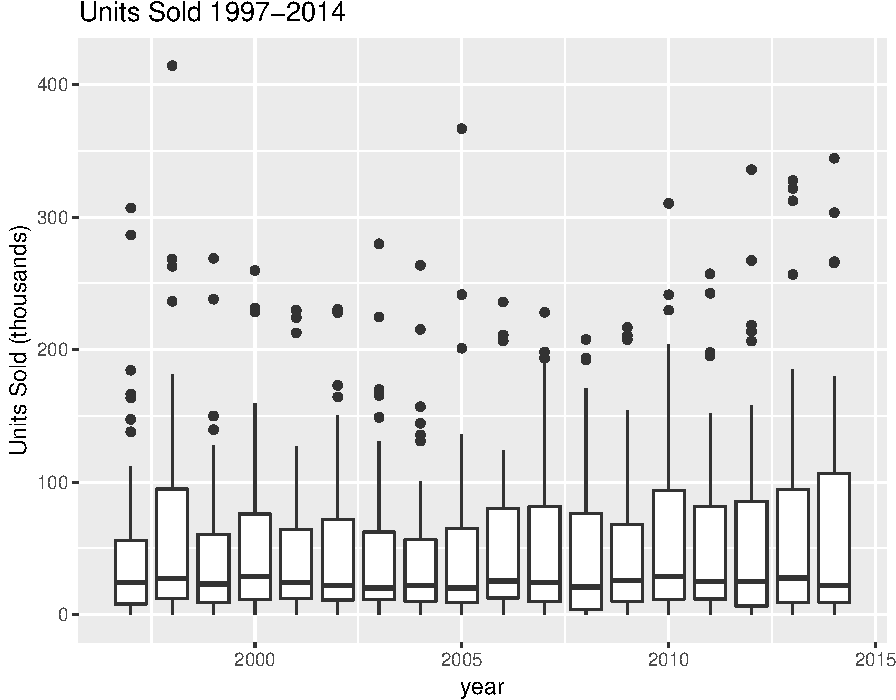
\includegraphics{Cultural_Exchange_and_Outbound_Migration_files/figure-latex/figl-1} \end{center}

The graph above shows distributions of units sold at different intitutes
for each year. As you can see the median stays mostly constant, although
with highly variable right tails.

\subsection{Independent Variable: Goethe Institute
Openings}\label{independent-variable-goethe-institute-openings}

In addition to the course units used, one can also look to see if there
is an increase in migration during times in which a GI is opened in a
country. This statistic is also found in the Goethe Institute data
abroad provided by @Übelmesser. In the data set, a date is given for
when an institute opens or closes, up to a maximum of three times in the
history of the specific institute. Using this data, we can look to see
how the migration changes at the time this happens.

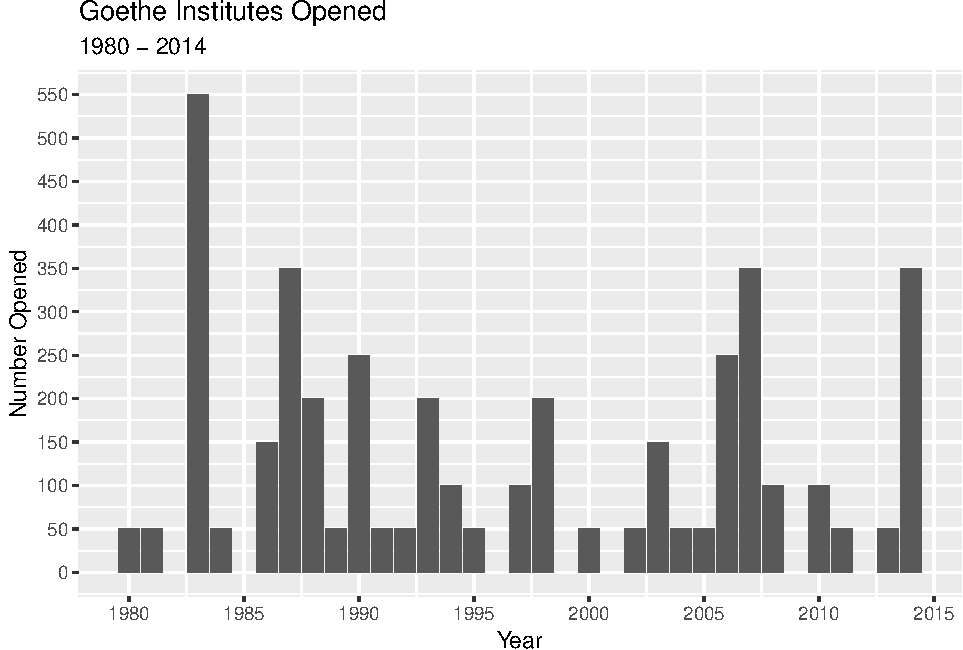
\includegraphics{Cultural_Exchange_and_Outbound_Migration_files/figure-latex/unnamed-chunk-2-1.pdf}

\subsection{Independent Variable:
Controls}\label{independent-variable-controls}

As there are many reasons that a person would choose to migrate to a new
country, several controls are needed. The first of which is to control
for the GDP of the destination country.

\section{Methodology}\label{methodology}

To begin with, a standard fixed effects model was applied to see if

\[ y_{jt} = \beta X_{jt} + \mu_{jt} \text{ for } t = \text{1997, 1998, ...,  2014} \text{ and } j =  \textit{country of destination} \]

\[y_{jt} = \alpha ^{\prime}X_{jt} + \phi ^{\prime} d_t  + \phi ^{\prime} d_j + \lambda \tilde{z}_{jt} + \eta_{jt}\]
with the weighted cross sectional averages defined as
\[\tilde{z}_{jt}= \frac{1}{\Sigma_j \omega_{jt}}(\sum_{j}\omega_{jt}y_{jt}, \sum_{j}\omega_{jt}x_{jt})\]

\section{Results}\label{results}

\section{Conclusions}\label{conclusions}

\section{References}\label{references}


\end{document}
